\section{Basic Analysis}
\label{891_2:sec:anal}

To quantify uncertainties in our full spectrum fitting methods we will
test different methods of fitting spectra and interpreting the
results. In this section we describe the basic, high-level methodology
that is common to all fitting methods. We also detail prepatory
analysis that is required before these methods can be applied to our
data, namely determining the velocity of each aperture and correcting
for Balmer emission.

%+++++++++++++++++++++++++++
%% {\bf MAB: Itemize (not in bullets, in sentences, clauses) the detailed
%%   preparatory analysis you will be describing. ``running the data
%%   through full spectrum fitting'' should be re-worded.

%------------------------
%% You should also have some preliminary discussion about why you are
%% laying the basics on the ``SSP fitting methodology.'' (I would call it
%% SPS not SSP, i.e., your SPS involves adding together SSPs.) For
%% example, there are the issues of degeneracies between age, metallicity
%% and extinction. There is also the issue of assumptions about the SFH
%% on $\tau_L$ and $Z_L$ for which the data cannot offer resolution,
%% i.e., the data does not allow you to know about the detailed SFH for
%% the older stellar populations. In other words, what is going to lead
%% you ultimately to the DFK approach. Foreshadow this.}

\subsection{SSP fitting methodology}
\label{891_2:sec:SSP_method}

Our fitting method involves minimizing differences between measured
NGC 891 spectra and synthetic galaxy spectra constructed from the
superposition of simple stellar populations (SSPs, see
\S\ref{891_2:sec:SSP_sets}). Fits are performed with
MPFITFUN\footnote{available at \url{http://purl.com/net/mpfit}}
\citep{Markwardt09}, an IDL implementation of the MINPACK Levenberg
Marquardt minimization algorithm \citep{More78}. The model galaxy
spectra are defined as
\begin{equation}
\label{891_2:eq:SSP_galaxy}
g(\lambda) = R(\lambda,\tau_V) \sum_{i,j} M(\Delta t_i,Z_j)
f(\lambda,\Delta t_i, Z_j),
\end{equation}
where $f(\lambda, \Delta t_i, Z_j)$ is the spectrum of an SSP with
metallicity $Z_j$ formed over time interval $\Delta t_i$, $M(\Delta
t_i,Z_j)$ quantifies the strength of the contribution of each SSP, and
$R(\lambda, \tau_V)$ governs the total extinction in the galaxy. All of our
SSPs are normalized to \val{1}{\sol{M}} so the strength of each SSP is
simply
\begin{equation}
\label{891_2:eq:fit_weight}
M(\Delta t_i,Z_j) = \int_{\Delta t_i} \psi(t, Z_j) dt,
\end{equation}
where $\psi(t, Z_j)$ describes the mass of stars formed at time $t$
with metallicity $Z_j$ (i.e., the star formation rate). In other
words, $M(\Delta t_i,Z_j)$ is the total mass in stars formed during
the time interval, $\Delta t_i$, associated with a particular SSP. The
extinction $R(\lambda, \tau_V)$ is parametrized by a single variable,
$\tau_V$ and, importantly, does not depend on SSP age ($t_i$) or
metallicity ($Z_j$). In \S\ref{891_2:sec:extinction} we discuss the details
of $R(\lambda, \tau_V)$ and the limitations of this
simplification. During fitting the free parameters are the SSP
weights, $M(\Delta t_i,Z_j)$, a single extinction term, \tauV, and the
systematic velocity.

%+++++++++++++++++++++++++++++
%% {\bf MAB: You should reference Levenberg Marquardt but I do not think
%%   you need to describe your coding language or the implementation in
%%   MPFITFUN. Concerning equation (1), you need to mention here what is
%%   being assumed given the placement of R. You can discuss it more
%%   later (in 3.3), but you should at least note the implications here
%%   and point to that later discussion here.}

For each aperture our primary values of interest are the age,
metallicity, and extinction. We measure extinction directly as $A_V =
1.086\ \tauV$, but age and metallicity depend on assumptions made
during fitting (i.e., priors in the SSP library) and during subsequent
analysis.

As shown in Equation \ref{891_2:eq:fit_weight} the fit weights describe the
integral of a particular star formation history (SFH), but it is
useful to reduce a SFH down to single values for age and
metallicity. To do this we define a pair of light-weighted
quantities. The mean, light-weighted age is
\begin{equation}
\label{891_2:eq:MLWA}
\tau_L = \frac{\sum_{i,j} W_{L,i,j}\times t_i}{\sum_{i,j} W_{L,i,j}}
\end{equation}
where $t_i$ is the age associated with each SSP and $W_L$ is the
``light weight'', defined as
\begin{equation}
\label{891_2:eq:light_weight}
W_{L,i,j} = M(\Delta t_i,Z_j)\sum_k S(\lambda_k) R(\lambda_k, \tau_V)
f(\lambda_k, \Delta t_i, Z_j),
\end{equation}
where $S(\lambda_k)$ defines a bandpass over which the light weight is
computed. We set $S(\lambda_k)$ to be flat over \val{5450}{\AA}
$\leq\lambda\leq$ \val{5550}{\AA} and zero everywhere else. The choice
of $t_i$ depends on assumptions about the SFH and in this work we make
the simple assumption that star formation is constant across the
lifetime of each SSP ($\Delta t_i$) so that $t_i$ is simply the
midpoint of each $\Delta t_i$. In \S\ref{891_2:sec:sys_err} we discuss and
quantify the systematics that arise from such an assumption. Similarly
to $\tau_L$ we also define the mean, light-weighted metallicity as
\begin{equation}
\label{891_2:eq:MLWZ}
Z_L = \frac{\sum_{i,j} W_{L,i,j}\times Z_j}{\sum_{i,j} W_{L,i,j}}.
\end{equation}

We note that Equation \ref{891_2:eq:light_weight} also describes a
conversion from mass-weights (i.e., $M(\Delta t_i, Z_j)$) to
light-weights that is simply a constant that is independent of the
specific mix of SSPs (but does depend on the overall extinction).

%+++++++++++++++++++++++
%% {\bf MAB: In eqn (4) move M outside of the sum since it does not
%%   depend on wavelength to clearly indicate that the factor between the
%%   light weight and the mass (weight) is a contant factor that depends
%%   on age and metallicity for a given band-pass. And say as much.}

\subsection{Velocities}
\label{891_2:sec:vel}

\begin{figure*}[t]
  \centering
  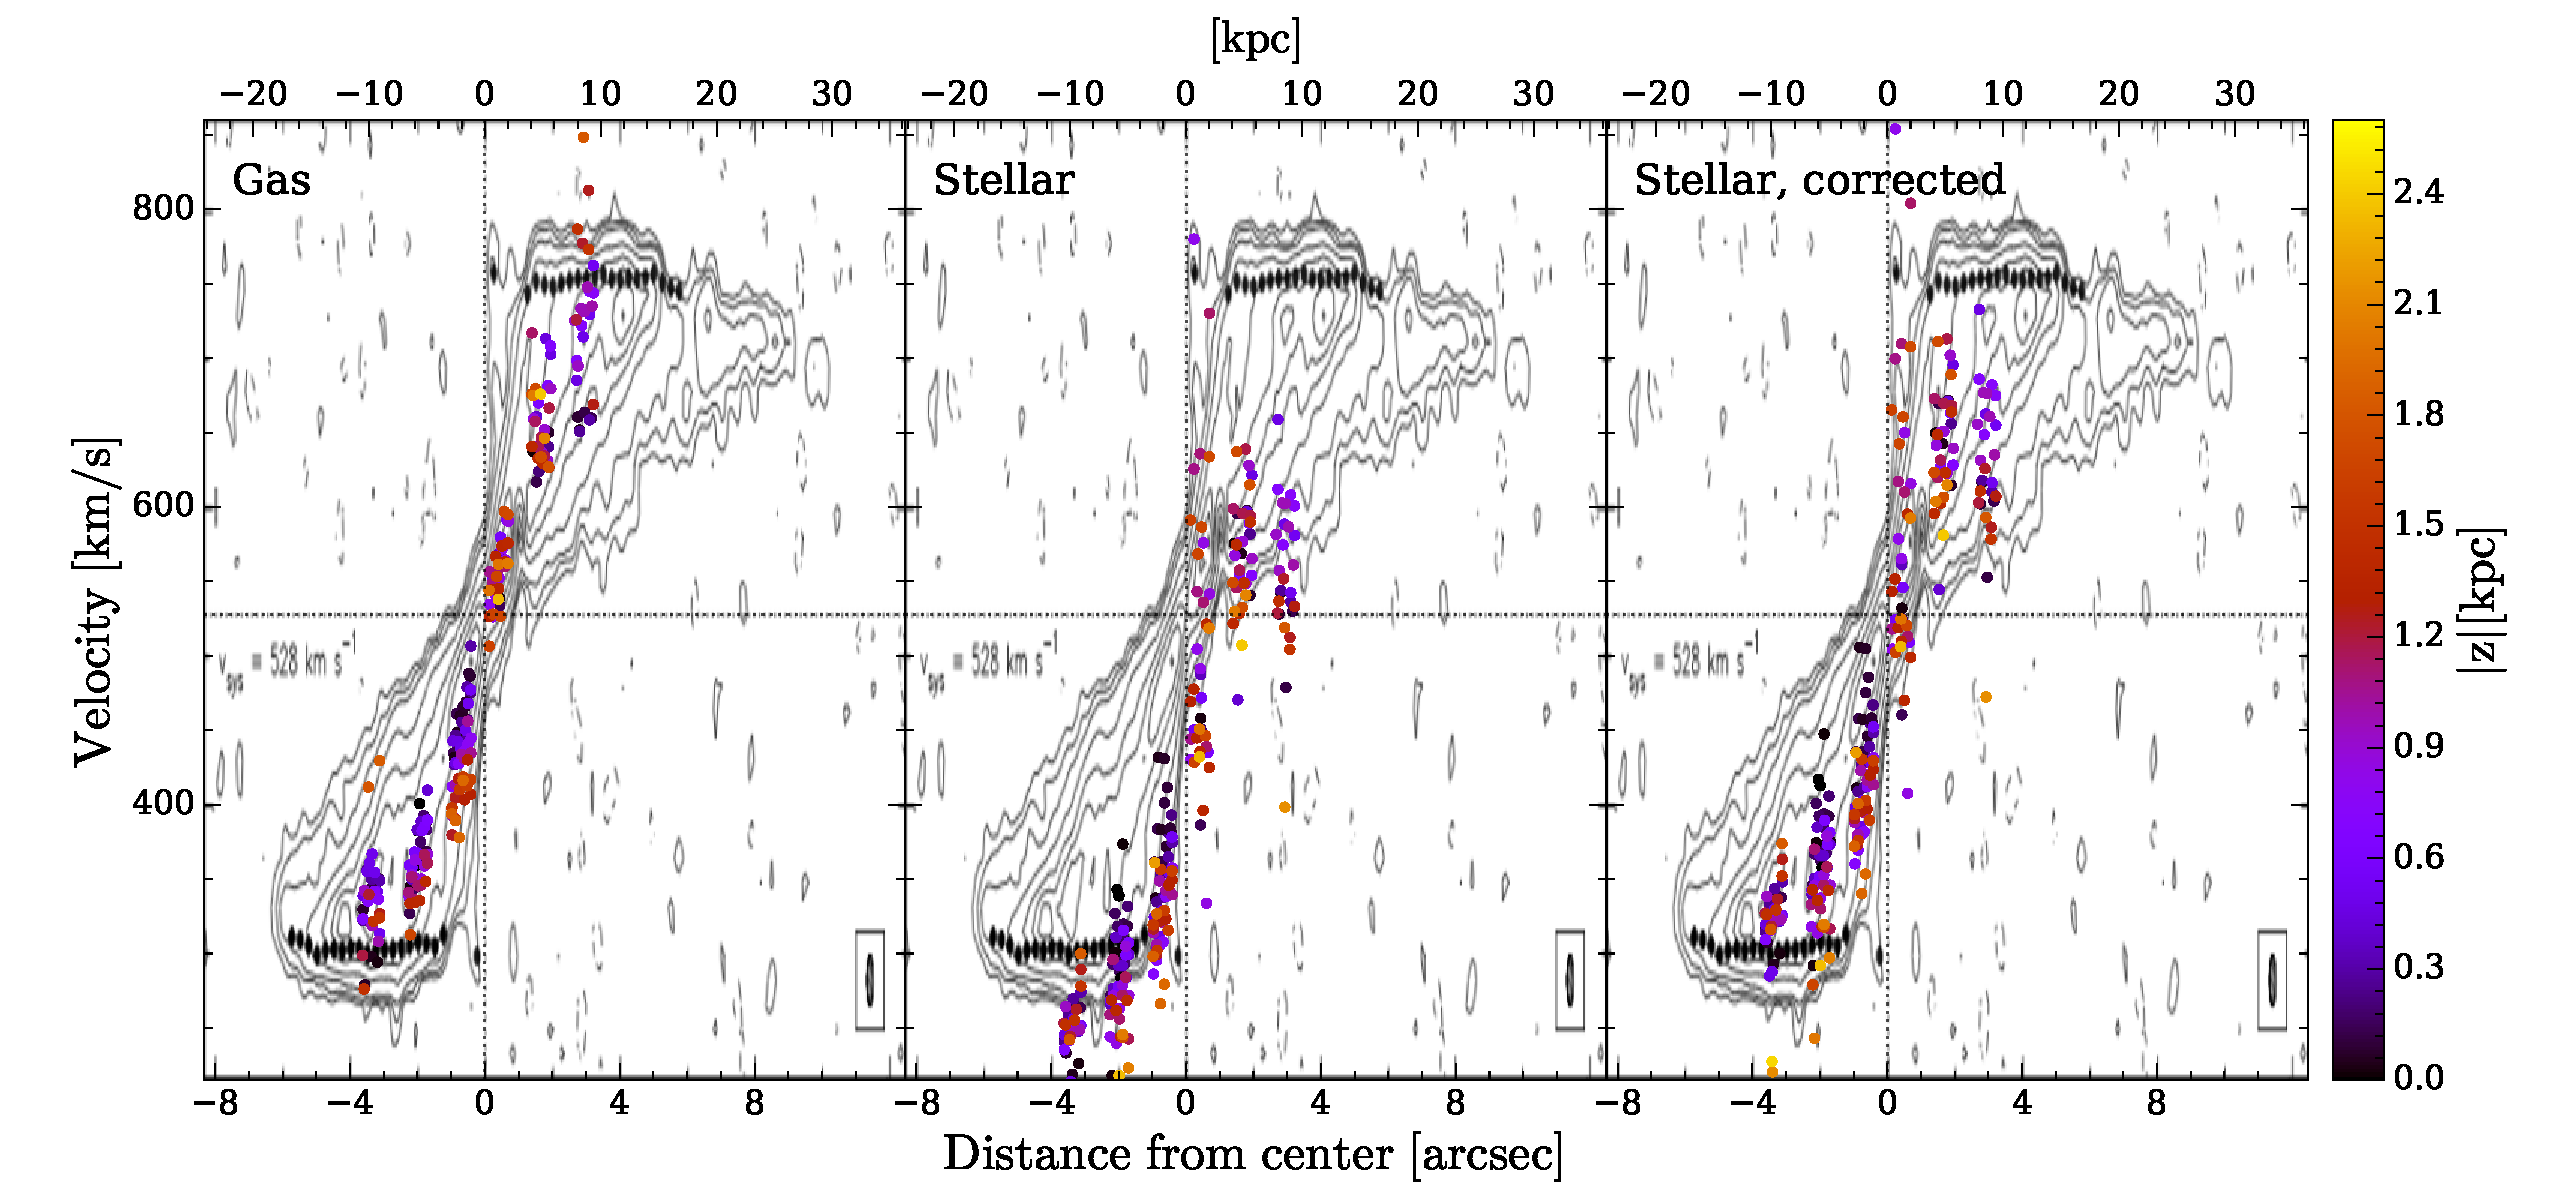
\includegraphics[width=\textwidth]{891_2/figs/Swat_vel.pdf}
  \caption[Comparison of measure stellar and gas velocities to HI
    velocity data]{\fixspacing\label{891_2:fig:Swat_vel}Comparison of
    HI velocity envelope (from \citet{Swaters97}) to \emph{left:}
    measured H$\alpha$ centroids, \emph{middle:} best fit velocities
    from SSP models, and \emph{right:} best fit stellar velocities
    with a constant offset to minimize median difference between gas
    and stars.}
\end{figure*}
The systemtic velocities of our model spectra do not depend on the
shape of the spectra (i.e., the SSP mix) and thus we can reduce the
number of free parameters in our SSP fits by measuring the velocities
once and then keeping them fixed for all subsequent analysis. The
final velocity values are a combination of velocity estimates from two
sources: the ``fit'' velocities that result from SSP fitting, and
velocities measured from the centers of bright emission lines.

%++++++++++++++++++++++
%% {\bf MAB: Do you mean ``systematic velocities'' or do you mean
%%   ``systemic velocities'' or ``line of sight velocities'' ? At the end
%%   of the paragraph enumerate in words what the following two
%%   subsubsections are.}

\subsubsection{Fit velocities}
During full spectrum fitting the velocity can be a free parameter of
the model, and this fit provides the first estimate of the velocity of
each aperture. The first step is to run a fully unconstrained fit
where all SSP weights, the velocity, and the extinction are allowed to
vary (see \S\ref{891_2:sec:SSP_method}. This produces a ``best fit'' only in
the sense that the resulting model spectrum matches the data well in a
$\chi^2$ sense; to determine velocities the details of the
astrophysical assumptions behind each model are unimportant. The
velocities found during fitting are generally precise on the order of
\val{\asim10}{\kms}, depending on \GP fiber size (see
\ref{chap:891_1}), which is slightly better that 10\% of the
instrumental resolution (again, depending on fiber size).

%++++++++++++++++++
%% {\bf MAB: Discuss the centroiding accuracy in terms of the
%%   instrumental resolution.}

Once the ``best fit'' spectrum is determined we run a second iteration
of the fitting routine with the SSP weights and extinction fixed to
the best fit values. This keeps the shape of the model spectrum the
same and causes $\chi^2$ minimization to be driven only by the
velocity offset between the model and the data. When fitting these
velocities we used only the range of wavelengths that lie within the
region spanned by arc lamp lines ($\val{4100}{\AA} \leq\lambda\leq
\val{6600}{\AA}$). This avoids wavelengths that could be affected by
extrapolation of the wavelength solution (see
\ref{chap:891_1}). In the majority of apertures this
``refined'' velocity was within \val{\asim 10}{\kms}, which is similar
to the precision of the fits and indicates that this second iteration
is perhaps not necessary.

%+++++++++++++++=
%% {\bf MAB: How important is this iteration? Again, compare amplitude of
%%   the change in the iteration to the instrumental resolution.
%% Refer to Paper-I concerning the wavelengths spanned by arcs (at the end of
%% the last sentence of the par.
%% }

The results of these fits produce what we call the ``fit
velocities''. The final fit values were found to be stable to a wide
(\val{\asim 100}{\kms}) range of starting velocity values. These
velocity fits are driven mainly by regions of the spectrum that
deviate significantly from the continuum level, which in our case are
the Balmer absorption series, the MgI absorption band, and the G
band. Many apertures show moderate to strong \Ha emission, but we
masked this feature (and [OIII]) during fits because our model SSPs do
not have nebular emission. For this reason the $\chi^2$ velocities can
be though of as the ``stellar'' velocity values.

%% {\bf MAB: Do you mask the upper Balmer series, including H-beta? I
%%   would have thought this would be important, and I thought you did.}

%% Comment for MAB: we actually didn't mask \HB. In retrospect maybe we
%% should have, but it is a rare aperture indeed that has strong enough
%% \HB emission to really mess with the residuals. Besides, the other
%% strong absorption features are certainly enough to simply fit a
%% centroid.

\subsubsection{Emission line velocities}

As a check on the velocities found above we also measure the velocity
of nebular emission lines, namely \Ha. Centroids were computed using
the IRAF task FITPROFS which allows us to deblend the \Ha, [NII]
complex. We focus only on the \Ha velocities, which are then compared
to known HI velocities from \citet{Swaters97}, as shown in the left
panel of Figure \ref{891_2:fig:Swat_vel}. We call the velocities measured in
\Ha ``gas velocities''.

%+++++++++++++++=
%% {\bf MAB: While I am ok with us comparing to Swaters+97 in Figure 1,
%%   are you taking into account in all of this analysis the trend in the
%%   HI tangential speed with height found in Oosterloo+07? This is
%%   essential I think. Last sentence are you measuring \Ha velocities or
%%   \Ha+[NII] velocities?}

The center panel of Figure \ref{891_2:fig:Swat_vel} shows the ``stellar
velocities'' compared to known HI velocities and our measured \Ha
velocities. Clearly there is a systematic offset between the stellar
and gas velocities that is relatively constant across both sides of
the galaxy. We find that this offset is constant in magnitude and sign
across both sides of the galaxy. This fact rules out an offset caused
by asymmetric drift \citep{Binney87}. Furthermore, many of the stellar
velocities are unphysical in the sense that they lie outside of the HI
envelope. We therefore conclude that this offset is caused by
systematic measurement uncertainty (likely arising from uncertainty in
our wavelength solution) and compute a constant velocity ``correction''
that is applied to the stellar velocities. This offset is computed to
minimize the median difference between stellar and gas
velocities. While we expect the stellar tangential speed to lag behind
the gas since we measure both sides of the galaxy, the median
difference between gas and stars should be, to first order, zero.

%+++++++++++++++++++++
%% {\bf MAB: I made a few edits in the above par. As part of or before
%%   the sentence beginning ``Clearly, ...'', add a description of what
%%   you see in Figure 1 that is clearly unphysical, i.e., the negative
%%   velocities in the middle panel below the gas. More broadly, discuss
%%   first the distribubtion of the ionized gas velocity w.r.t. the
%%   envelop from HI. This envelop should be noted in the text and the
%%   figure caption. Explain why we might expect the ionized gas to lie
%%   below the HI envelop, i.e., we are measuring a centroid. What should
%%   the reader make of the few points in the upper part of the left
%%   panel that are above the HI envelope? Are these bad measuremets? Add
%%   error bars?

%%   Define AD -- you can reference Binney \& Tremaine.

%%   Discuss what the soures of possible uncertainty could be in the
%%   stellar velocities. Is this a problem with the wavelength solution
%%   -- something that you come to in the next paragraph, or something
%%   else? Did you check that the wavelength solution and the BC03
%%   templates were either both in vacuum or air?

%---------------------
%%   Lastly, concerning the use of the median, yes, maybe to to zeroth
%%   order the median difference should be zero, but not to a \kms
%%   level. The median difference is going to depend on at least the
%%   number of points on the positive and negative sides of the galazy to
%%   zeroth order. To first order it will depend on the radial
%%   distribution particularly near the center where the projected
%%   velocity is small. Can you address this?}

\begin{figure}[t]
  \centering
  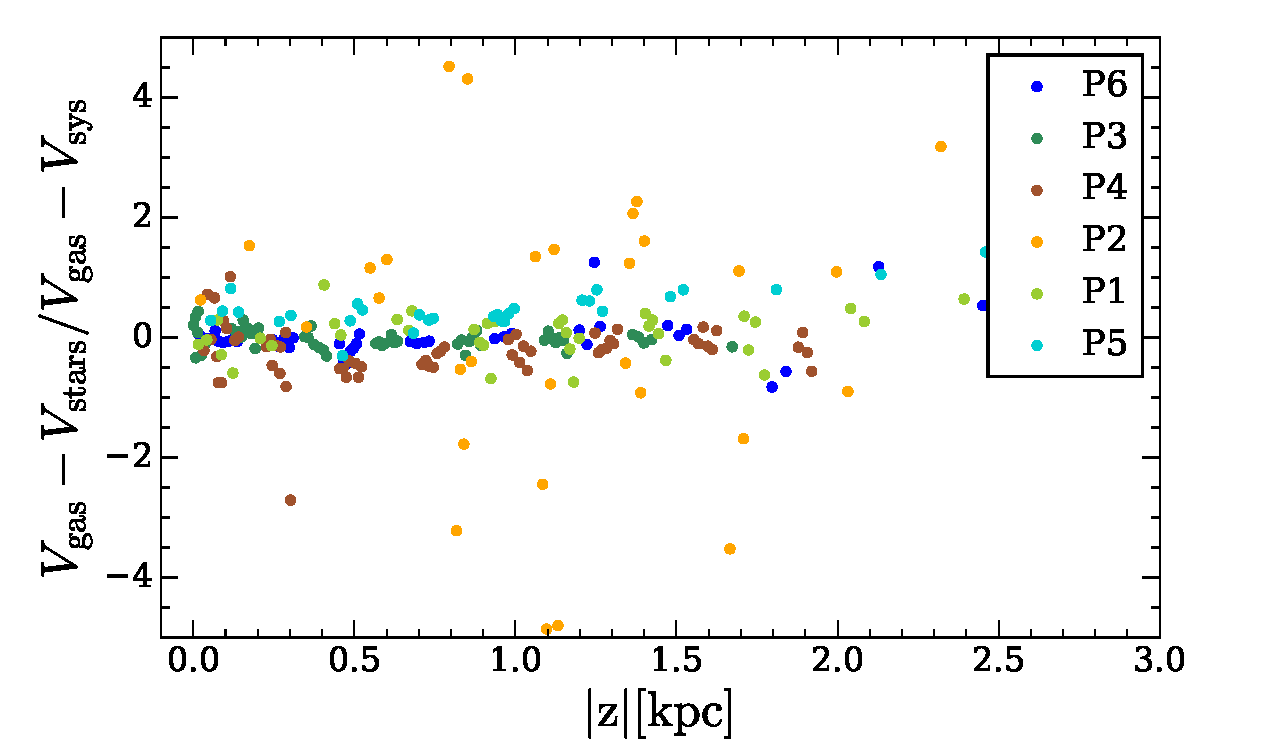
\includegraphics[width=\columnwidth]{891_2/figs/SG_diff.pdf}
  \caption[Offset between stellar and gas
    velocities]{\fixspacing\label{891_2:fig:SG_offset}Difference
    between stellar and gas velocities after applying a constant
    \val{74}{\kms} offset to the stars. A median of 1 corresponds to
    no average offset between the two population \emph{across both
      sides of the galaxy}.}
\end{figure}

Figure \ref{891_2:fig:SG_offset} shows the relation between stellar and gas
velocities after applying an offset of \val{74}{\kms}. Based on these
results, the final velocity of each aperture is fixed as the velocity
measured during $\chi^2$ fitting (``stellar velocity'') plus a
constant offset of \val{74}{\kms}. The right hand panel of Figure
\ref{891_2:fig:Swat_vel} shows the final velocities used. We note that the
systematic correction of \val{74}{\kms} is within the total
uncertainty in our velocity as dictated by uncertainties in the
wavelength solution (\val{120}{\kms}, see \ref{chap:891_1}).

%+++++++++++++++++++=
%% {\bf MAB: The standard is km s$^{-1}$ not \kms. At the end here you
%%   want to discuss the difference between the stars and gas in the left
%%   and right panels compared to each other and the HI envelop. For
%%   example, the asymmetry in the stars is not seen in the gas.}

\subsection{Extinction Model}
\label{891_2:sec:extinction}

During full spectral fitting (\S\ref{891_2:sec:SSP_method}) we assume the
extinction model of \citet{Charlot00} during all analysis steps, which
is described by
\begin{equation}
R(\lambda) = e^{-\tauV \left(\lambda/\val{5500}{\AA}\right)^{-0.7}}.
\end{equation}
This model has a steeper slope than a simple foreground dust screen,
but the authors show it accurately reproduces the ratio of
far-infrared to ultraviolet luminosities, the ratio of \Ha to \HB
luminosities, the \Ha equivalent width, and the ultraviolet spectral
slope of nearby starburst galaxies. We retain the functional
dependence of $\tau \propto \lambda^{-0.7}$ and define two
normalizations, one for gas emission and one for stellar
continuum. Thus, the total optical depth to a particular species is
either
\begin{equation}
\tau_{{\rm cont}}(\lambda) = \tauV \left(\frac{\lambda}{\val{5500}{\AA}}\right)^{-0.7}
\end{equation}
or
\begin{equation}
\label{891_2:eq:tauVB}
\tau_{{\rm em}}(\lambda) = \tauVB \left(\frac{\lambda}{\val{5500}{\AA}}\right)^{-0.7},
\end{equation}
where \tauV and \tauVB are the normalization factors for stellar continuum and
gas emission, respectively.

As described in \S\ref{891_2:sec:SSP_method}, \tauV is a free parameter of
the SSP models that essentially measures the slope of the
continuum. To measure \tauVB we use the ratio of measured \Ha/\HB flux
and compare it to the expected value of 2.86 from
\citet{Osterbrock89}, assuming case B recombination in a \val{10^4}{K}
gas. Under these assumptions, and given the extinction law in equation
\ref{891_2:eq:tauVB}, we compute
\begin{equation}
\label{891_2:eq:Balmer_extinction}
\tauVB = 4.84 \ln \left(\frac{\Ha/\HB}{2.86}\right).
\end{equation}

The \Ha and \HB line fluxes were measured using the IRAF task FITPROFS
which allows us to deblend the \Ha/[NII] emission feature. Before
fitting the emission lines a ``best fit'' galaxy model is
subtracted. As in \S\ref{891_2:sec:vel} the detailed astrophysics of the
best fit model are unimportant; we only require that the model
accurately match the stellar continuum so that it can be subtracted
from the data. Once the continuum is subtracted the data are smoothed
with a 3 pixel (\val{\asim 350}{\kms}) wide moving average. To
mitigate the impact of bad continuum fits the centroid fitting window
is constrained to be only $\sim 4\sigma$ wide, where $\sigma$ is the
average spectral width (standard deviation) of bright sky emission
lines.

%++++++++++++++++++==
%% {\bf MAB: In the first sentence above do you mean SSP or SPS? I think
%%   the latter. Concerning the 600 \kms wide moving average, is this
%%   equivalent to a boxcar of xx pixels? If so, you might say ``the data
%%   are smoothed with a 600 km s$^{-1}$ (XX pixel) wide moving average,
%%   or boxcar.'' Again, modify \kms to km s$^{-1}$. However, I am not
%%   sure I understand the need for this smoothing and how it reduces the
%%   impact of bad continuum fits. Why? It seems to me you will make the
%%   NII+Ha blending worse which also sounds like it is a problem.}

The relative strength of the two [NII] lines in the \Ha/[NII] complex
is governed by quantum mechanics and we expect the flux ratio
[NII]$_{6585}$/[NII]$_{6549} = 3$. When measuring the \Ha/[NII] lines,
however, we often find [NII]$_{6585}$/[NII]$_{6549} > 3$, which
indicates that the line fit is attributing some of the [NII]$_{6549}$
flux to \Ha and causing the \Ha flux to be overestimated.  This is
likely due to an incorrect de-blending of the \Ha and [NII]$_{6549}$
lines.  We correct for this effect by using the flux of [NII]$_{6585}$
as a ``calibration'' flux (reasonable given its isolation, away from
blending issues of \Ha and [NII]$_{6549}$) and define an \Ha
correction,
\begin{equation}
  \label{891_2:eq:balmer_corr}
  \Delta\Ha = \mathrm{[NII]}_{6549} - \frac{\mathrm{[NII]}_{6585}}{3},
\end{equation}
which is added to the measured \Ha flux.

As mentioned above, measuring \Ha and \HB emission requires first correcting
for \Ha and \HB absorption present in the stellar continuum. In practice the
entire process is iterative because fitting SSPs accurately requires accurate
emission corrections (\S\ref{891_2:sec:emission_corr}), which, in turn, requires
accurate extinction values. We find that the measured Balmer fluxes
and derived emission corrections are stable after only a single
iteration.

%+++++++++++++++
%% {\bf MAB: I would like to understand the issue with the imperfect
%%   continuum subtraction (in the sentence ``This is likely due...'')
%%   and how it alters the NII ratio. In this paragraph, leading up to
%%   the motivation for eqn 10 you want to say that the concept here is
%%   to trust the 6585 NII line because of its greater wavelength
%%   separation from Ha. However, you also need to address wy you think
%%   the continuum subtraction is better for 6585, i.e., why for some
%%   reason the baseline for this line isn't what is causing the problems
%%   with the ratio not equalling 3. 

%-----------------
%%   Further, you need to provide the
%%   amplitude of the correction which I expect will vary significatly
%%   with Ha line-strength and height (NII/Ha changes). So I'd like to
%%   know the \% correction to the Ha flux in the mean (and/or median),
%%   and the trends with height, e.g., numbers for 0-0.4 kpc, 0.4-1 kpc,
%%   $>$1 kpc.}

\subsection{Emission Corrections}
\label{891_2:sec:emission_corr}

Many of our apertures show moderate to strong Balmer emission that is
not present in the SSP libraries that underlie our galaxy models and
therefore must be subtracted before accurate analyses can be made. To
do this we construct a model spectrum containing only emission from
\Ha, \HB, \Hg, \Hd, and \He.  The basic idea is to first construct a
model galaxy based on fits that mask the cores of the Balmer lines and
then use these fits to remove the stellar continuum and isolate the
Balmer emission. Then the two strongest emission lines (\Ha and \HB)
can be used to construct a model containing emission from the
higher-order lines.  Based on the results of \citet{Osterbrock89}, and
assuming case B recombination in a \val{10^4}{K} gas, the ratios of
fluxes for the Balmer series is \mbox{1 : 0.350 : 0.164 : 0.087 :
  0.056} (\Ha : \HB : \Hg : \Hd : \He). In our emission models the
width of each line is dictated by the instrumental resolution measured
at the line location (see \ref{chap:891_1}), with apertures
made from different sized \GP fibers having different widths.

%++++++++++++++++++++=
%% {\bf MAB: First sentence: I think you mean SPS models (that use
%%   SSPs). I'd like you to explain the notion behind the approach in an
%%   explicit way. The notion is an important idea. The kernel of it is
%%   that Hydrogen Balmer Case B emission strength decreases sigificantly
%%   with higher order, e.g., by more than a factor of 10 between
%%   H$\alpha$ and H$\delta$. In contrast, the equivalent width of the
%%   Hydrogen Balmer absorption in stellar photospheres does not display
%%   this trend, and indeed H$\alpha$ absorption EW is weaker than
%%   H$\beta$. This contrast can be used to our advantage in an iterative
%%   scheme that first masks the cores of the Balmer absorption lines
%%   where the emission is present to provide a first-order estimate the
%%   continuuum. Once subtracted, only the two strongest emission lines
%%   are used to estimate the normalization of the emission and the
%%   attenuation, from which the remaining line-emission is estimated.}

\begin{figure}
  \centering
  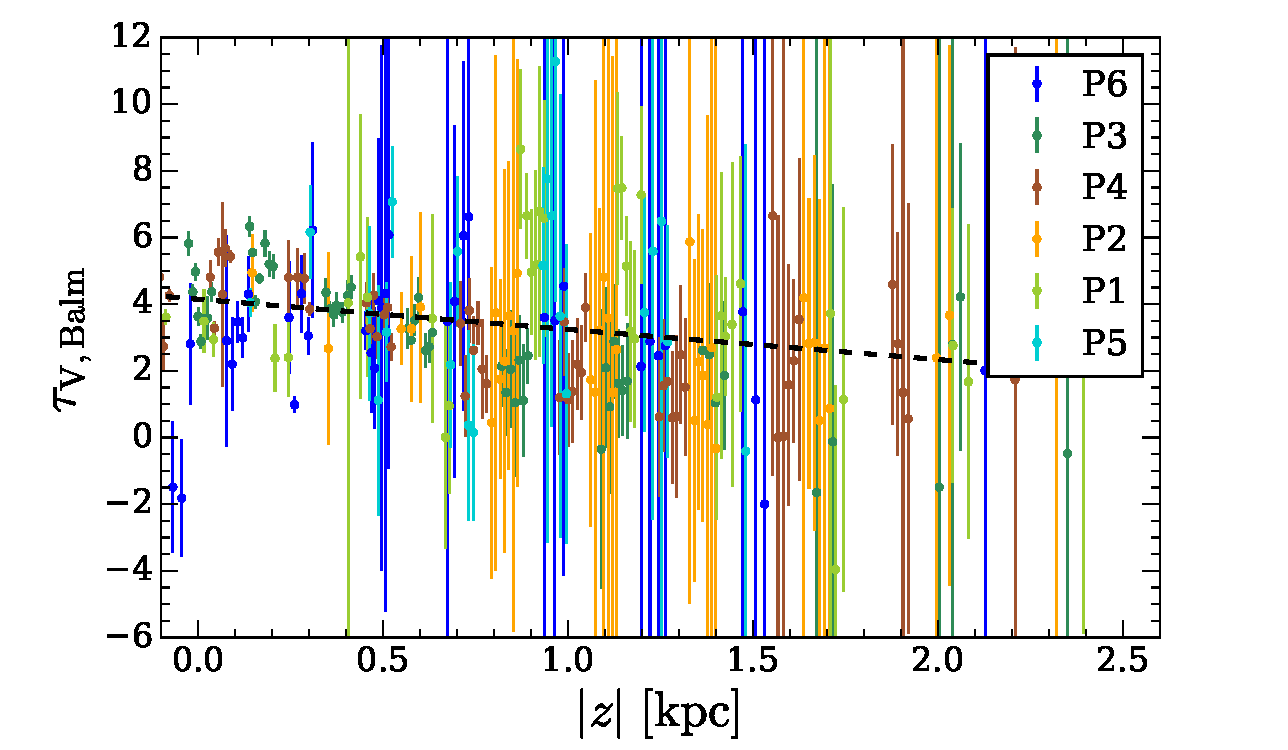
\includegraphics[width=\columnwidth]{891_2/figs/TauV_balm.pdf}
  \caption[Height dependendence of
    \tauVB]{\fixspacing\label{891_2:fig:tauVB_height}Measured values
    of \tauVB as a function of distance from the midplane. The error
    bars show the uncertainties reported by IRAF from 100 Monte Carlo
    noise iterations. The black shows a linear fit described in
    Equation \ref{891_2:eq:tauVbalm}.}
\end{figure}

This idealized Balmer emission model is then extincted using Equation
\ref{891_2:eq:Balmer_extinction} based on the value of \tauVB as measured in
section \ref{891_2:sec:extinction}. To minimize the impact of aberrant
extinction calculations we compute a height-dependent \tauVB by
fitting a line to the data from all apertures (and thus from all
radii), as shown in Figure \ref{891_2:fig:tauVB_height}. From these data it
is clear that the radial dependence to the vertical trend in \tauVB is
minimal so our grouping of all radii is valid. We find for NGC 891
\begin{equation}
\label{891_2:eq:tauVbalm}
  \tauVB (z) = -0.91 z + 4.15,
\end{equation}
which allows us to compute the extinction in our Balmer emission
models at any height above the midplane.

%----------------------
%% {\bf MAB: Concerning Figure 3: Yuck. I can't tell if the line is a
%%   good fit to the data and whether there is a radial dependence. (You
%%   should say ``a radial dependence to the vertical trend.'') Clearly
%%   we see a radial trend in the stellar absorption later so this result
%%   is somewhat puzzling without some thought and
%%   interpretation. Regarding the figure itself, I'd like to see a
%%   version w/o the error bars. The error bars must be wrong because
%%   they are far larger than the scatter. I would also like to see
%%   moving averages for all pointings as well as for individual
%%   pointings.}

\begin{figure}
  \centering
  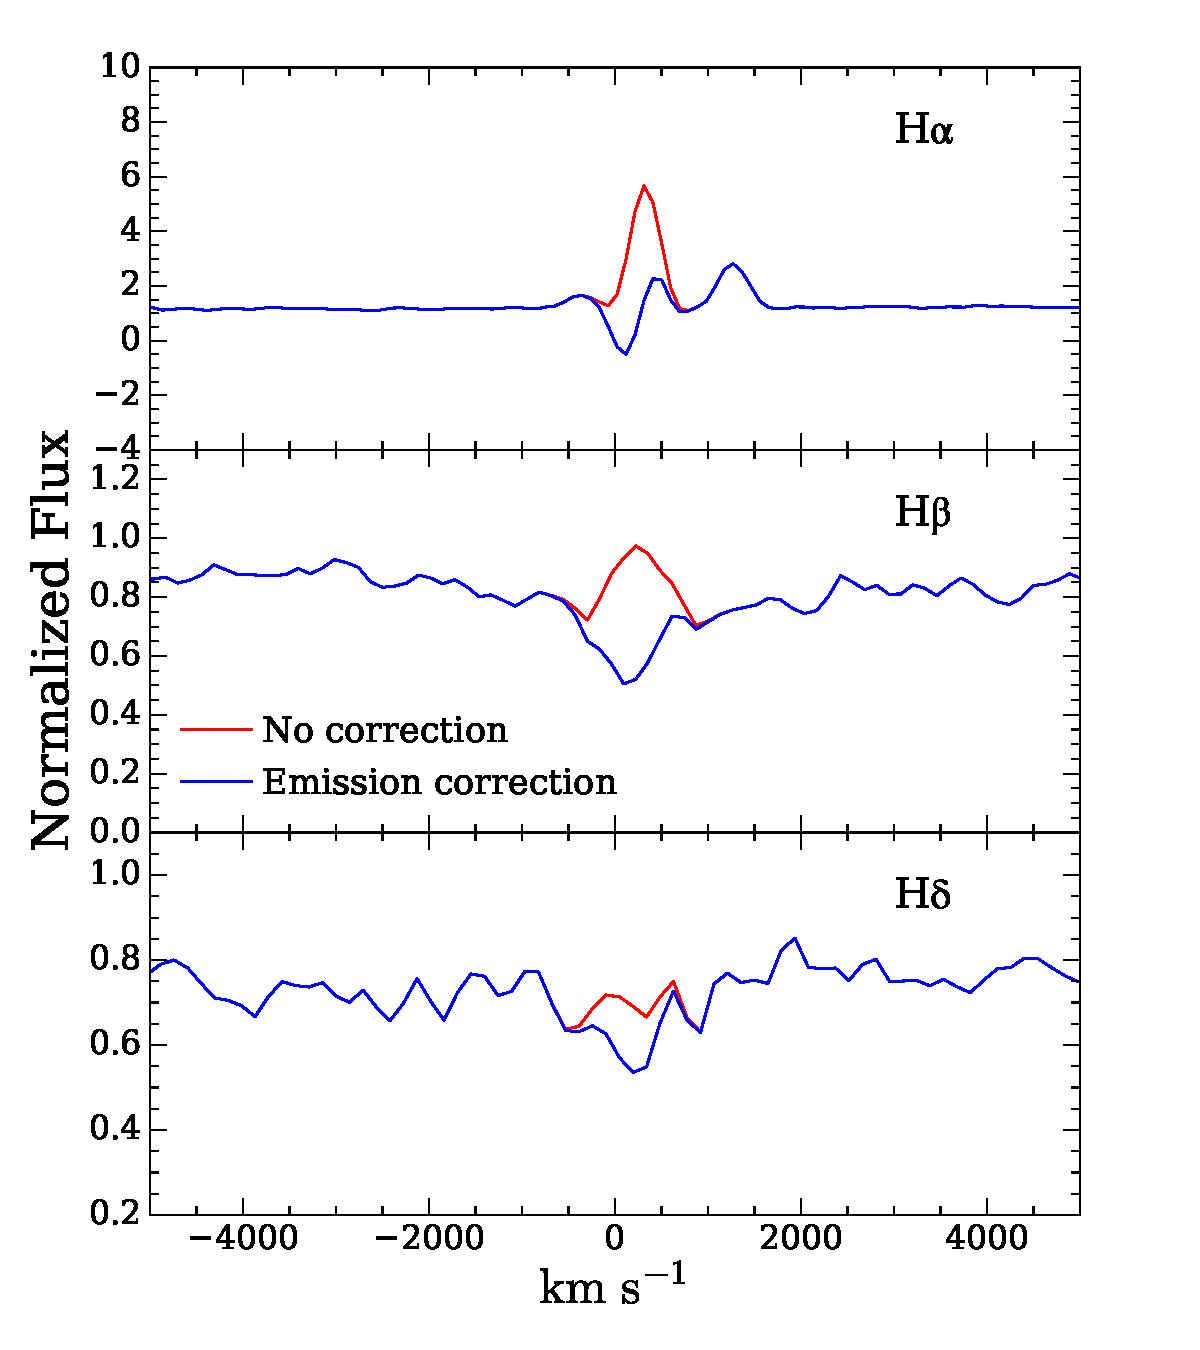
\includegraphics[width=\columnwidth]{891_2/figs/emission_comp_zoom.pdf}
  \caption[Spectra before and after Balmer emission
    correction]{\fixspacing\label{891_2:fig:emission_comp}An example
    of Balmer emission correction. The red and blue spectra show an
    aperture with strong Balmer emission (aperture P4.6) before and
    after the Balmer emission model described in
    \S\ref{891_2:sec:emission_corr} is applied.}
\end{figure}

Finally, the emission model is scaled so the \Ha flux matches the \Ha
flux measured in each individual aperture. The data spectra are then
corrected by subtracting the corresponding emission model. Figure
\ref{891_2:fig:emission_comp} shows an example of a spectrum with strong \HB
emission before and after subtracting the Balmer emission model. In
many apertures the blending of the \Ha/[NII] complex causes imperfect
subtraction in this region (as it should, our emission model does not
contain [NII] emssion), and in subsequent analysis we do not fit
(i.e., mask) data within \val{\pm 500}{\kms} of \Ha (which includes
both [NII] lines).

In addtion to \Ha/[NII] we mask other strong sources of nebular
emission ([OIII]$_{4959}$, [OIII]$_{5007}$, and S2) and sky lines with
strong residuals ([OI]$_{6300}$, NaD, and OI$_{5577}$).

%++++++++++++++++===
%% {\bf MAB: Itemize the lines that you mask -- all of them -- and give
%%   equivalent pixels to 500 \kms at the wavelength extrama. For Figure
%%   4 I can't see anything in this figure so I recommend you show
%%   blow-ups in wave for the Balmer lines from $\alpha$ to $\epsilon$.}

As mentioned above, the best-fit, extinction-value, emission-model
analysis steps are interconnected and at least one iteration is
required to find the ``final'' values.


